\section{LED kruh}

Trezoru vévodí světelný kruh. Slouží jako displej, na kterém trezor může zobrazovat vše, co potřebuje. Kruh obsahuje šedesát jednotlivých ledek 
\href{https://cdn-shop.adafruit.com/datasheets/WS2812B.pdf}{WS2812}, konkrétně WS2812 mini. Variantu mini jsem zvolil, aby kruh mohl mít menší
průměr, který takto vychází na 80~mm. WS2812 mají totiž rozměr pouzdra 3,5x3,5~mm, zatím co ostatní varianty mají rozměry 5x5~mm, což by znamenalo průměr kruhu alespoň 120~mm.

WS2812 není jen ledka, ale má v sobě logiku, díky které je možné je řetězit za sebe, takže na řízení celého kruhu stačí jen jeden pin na ESP32.\newline
Ukázka PCB viz obrázek \ref{fig:E4-LedDeska}.
\begin{figure}[htbp]
    \centering
    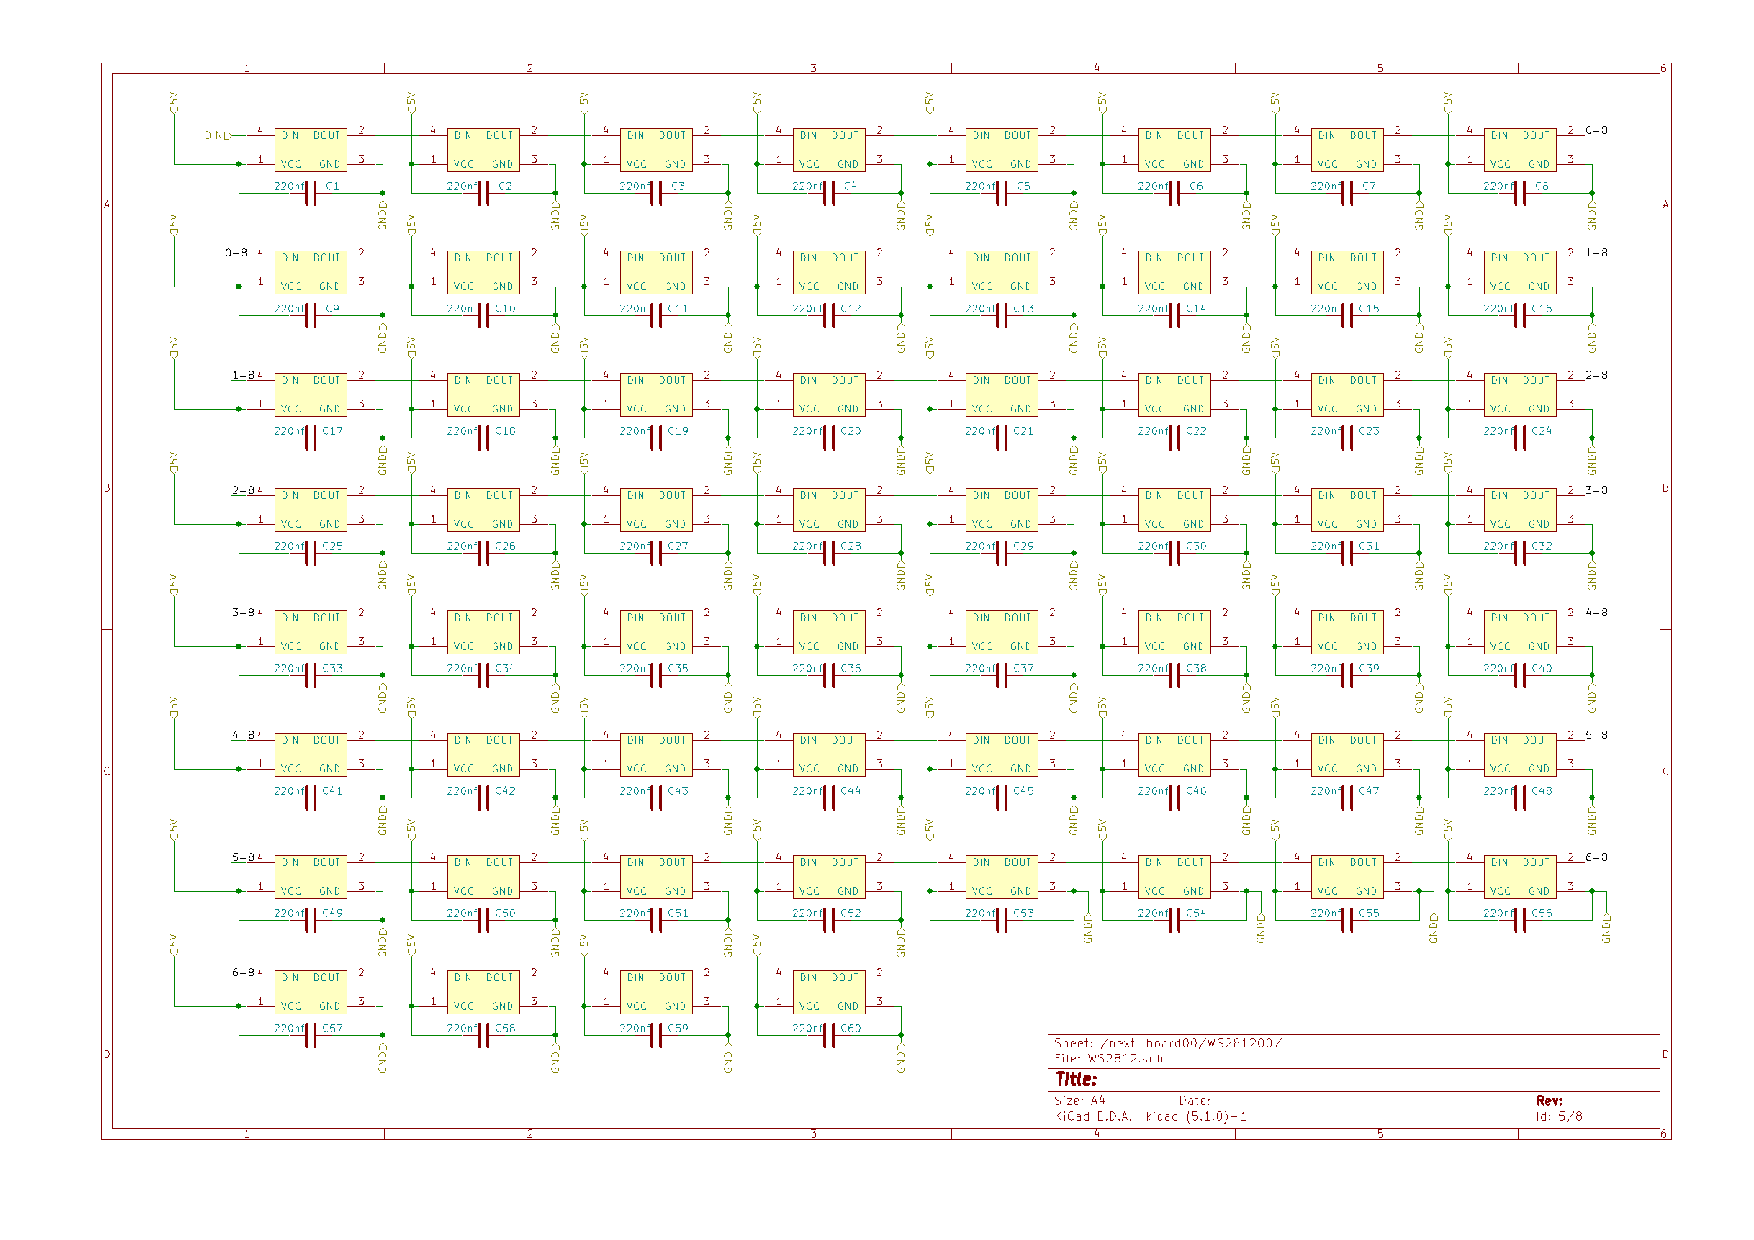
\includegraphics[width=\textwidth]{kapitoly/obrazky/E4/WS2812/zapojeni_WS2812.pdf}
    \caption{Zapojení ledek WS2812 na desce trezoru -- schéma}
    \label{fig:E4-sch_civka_tercik}
\end{figure}

\newpage